% !TEX root = ../discriminative_filtering.tex

\section{The Bernstein--von Mises Theorem} \index{Bernstein--von Mises theorem|(} 
For a random variable $\Theta\sim\operatorname{Uniform}([0,1])$, suppose we were to draw an infinite sequence of random variables
\[
X_1, X_2 \dotsc\sim^\text{i.i.d.}\operatorname{Bernoulli}(\Theta).
\]
Then:
\[
p(\theta | x_1,\dotsc, x_n)
\propto \theta^{n\bar x} (1-\theta)^{n(1-\bar x) } \mathds{1}_{[0,1]}(\theta)
\]
where $\bar x =  \tfrac{1}{n}\sum_{i=1}^n x_i$ so that $\Theta|X_1,\dotsc,X_n \sim \operatorname{Beta}(n\bar x+1, n(1-\bar x)+1)$.  This distribution has mode $\bar x$ and variance bounded by $1/(n+2)\to 0$.  The distribution of the prior on $\Theta$ is flat on $[0,1]$ and the distribution of $\Theta|X_1$ is a line on $[0,1]$, but quite quickly $\Theta|X_1,\dotsc,X_n$ looks bell-shaped, and vaguely Gaussian.   This is not a coincidence.  Loosely speaking, for any continuous random variable $\Theta$, if you draw a sequence $X_1, X_2 \dotsc$ of random variables that each provide a bit more information about $\Theta$, then $\Theta|X_1,\dotsc,X_n$ becomes Gaussian in the total variation metric.  

%%%%%%%%%%%%%%%%%%%%%%%%%%%%%%%%%%%%%%%%%%%%%%%%%
\begin{figure}
\begin{minipage}[c]{.45\textwidth}
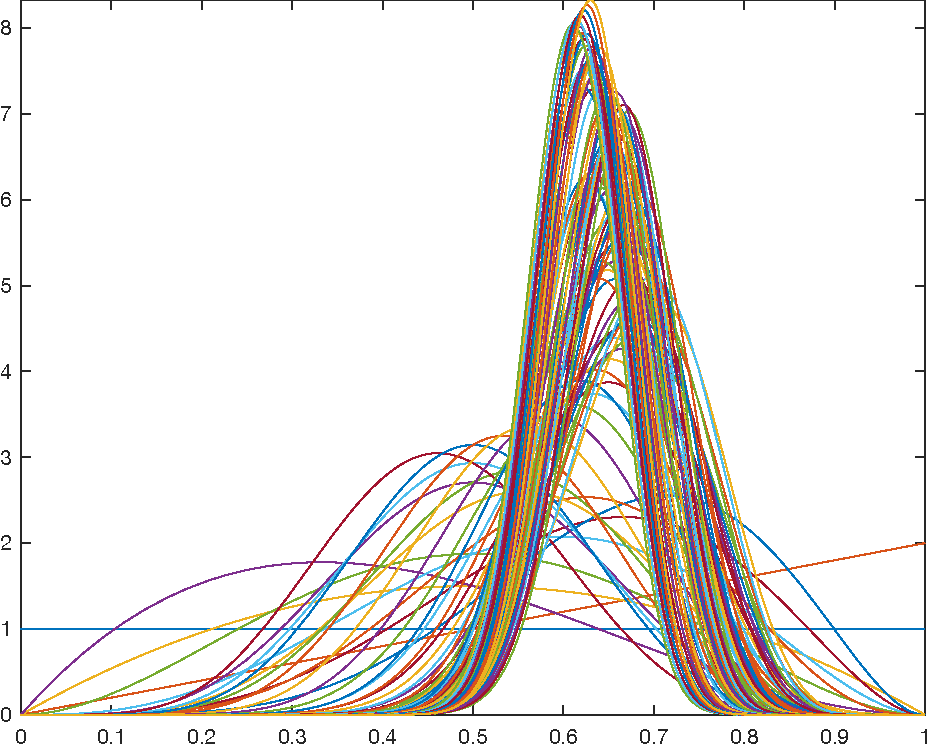
\includegraphics[width=\linewidth]{bvm_illustration}
\end{minipage}%
\hfill
\begin{minipage}[c]{.45\textwidth}
\caption[An Illustration of the Bernstein--von Mises Theorem]{I sampled $X_1,\dotsc,X_{100}\sim^\text{i.i.d.}\operatorname{Bernoulli}(0.6)$ and plotted the conditional densities $p(\theta|X_1=x_1,\dotsc,X_n=x_n)$ for $n=1,\dotsc, 100$ on the left.  The bell shape is well-established by $n=10$.}
\end{minipage}
\end{figure}
%%%%%%%%%%%%%%%%%%%%%%%%%%%%%%%%%%%%%%%%%%%%%%%%%

Strictly speaking, we quote the following theorem from \textcite{vdV98}:
\begin{quote}
\emph{Let the experiment $(P_\theta:\theta\in\Theta)$ be differentiable in quadratic mean at $\theta_0$ with nonsingular Fisher information matrix $I_{\theta_0}$, and suppose that for every $\epsilon>0$ there exists a sequence of tests $\phi_n$ such that:}
\[
P_{\theta_0}^n\phi_n \to 0, \quad
\sup_{\norm{\theta-\theta_0}\ge\epsilon} P_\theta^n(1-\phi_n) \to 0
\]
\emph{Furthermore, let the prior measure be absolutely continuous in a neighborhood of $\theta_0$ with a continuous positive density at $\theta_0$.  Then the corresponding posterior distributions satisfy}
\[
\norm{P_{\sqrt{n}(\bar\Theta_n-\theta_0)|X_1,\dotsc,X_n} - \N(\Delta_{n,\theta_0},I_{\theta_0}^{-1})}\xrightarrow{P_{\theta_0}^n} 0
\]
\end{quote}
where $\Delta_{n,\theta_0}=\tfrac{1}{\sqrt{n}}\textstyle \sum_{i=1}^n I_{\theta_0}^{-1} \dot{\ell}_{\theta_0}(X_i)$, $\dot{\ell}_{\theta_0}$ is the score function of the model, and the norm is that of total variation.  A test is defined as ``a measurable function of the observations taking values in the interval $[0,1]$.'' Total variation is invariant to location and scale changes, so it follows that
\[
\norm{P_{\bar\Theta | X_1,\dotsc,X_n} - \N(\hat\theta_n, \tfrac{1}{n} I_\theta^{-1})}\xrightarrow{P_\theta^n} 0.
\]
While this result can be used to justify statements along the lines of ``the prior does not matter in Bayesian inference as the amount of data becomes large,'' we use this result instead to argue that, under relatively general conditions, $Z_t|X_t$ will become Gaussian as $\dim(X_t)\rightarrow\infty$.  What follows now is justification for the argument that, if the conditions for the Bernstein--von Mises Theorem are satisfied, then the posterior computed by the DKF will become close to the true posterior in the total variation metric as $\dim(X_t)\rightarrow\infty$.
\index{Bernstein--von Mises theorem|)} 

%%%%%%%%%%%%%%%%%%%%%%%%%%%%%%%%%%%%%%%%%%%%%%%%%
\section{Proof of Theorem} \index{Discriminative Kalman Filter!proof of consistency|(}
Our main technical result is Theorem \ref{t:pn}. After stating the theorem we translate it into the setting of the paper. Densities are with respect to Lebesgue measure over $\mathbb{R}^d$. $\|\cdot\|$ and $\|\cdot\|_\infty$ denote the $L_1$ and $L_\infty$ norms, respectively, $\to$ denotes weak convergence of probability measures (equivalent, for instance, to convergence of the expected values of bounded continuous functions), and $\delta_c$ denotes the unit point mass at $c\in\mathbb{R}^d$.  Define the Markov transition density $\tau(y,z)=\eta_d(z;Ay,\Gamma)$, and let $\tau h$ denote the function
\[ (\tau h)(z) = \int \tau(y,z) h(y) dy \]
for an arbitrary, integrable $h$. Define $p(z)=\eta_d(z;0,S)$, where $S$ satisfies $S=ASA^\tr+\Gamma$. 
\begin{theorem} \label{t:pn}
 Fix pdfs $s_n$ and $u_n$ $(n\geq 1)$ so that the pdfs
\begin{equation} \label{e:pn-BF2} p_n = \frac{u_n\tau s_n/p}{\|u_n\tau s_n/p\|}  \end{equation}
are well-defined for each $n$. Suppose that for some $b\in\mathbb{R}^d$ and some probability measure $P$ over $\mathbb{R}^d$
\begin{enumerate}
\item[A1.] $s_n \to P$ as $n\to\infty$;
\item[A2.] there exists a sequence of Gaussian pdfs $(s'_n)$ such that $\|s_n-s'_n\|\to 0$ as $n\to\infty$;
\item[A3.] $u_n \to \delta_b$ as $n\to\infty$;
\item[A4.] there exists a sequence of Gaussian pdfs $(u'_n)$ such that $\|u_n-u'_n\|\to 0$ as $n\to\infty$;
\item[A5.] $p_n \to \delta_b$ as $n\to\infty$;
\end{enumerate}
Then
\begin{enumerate}
\item[C1.] $s'_n \to P$ as $n\to\infty$;
\item[C2.] $u'_n \to \delta_b$ as $n\to\infty$;
\item[C3.] the pdf
\[ p'_n = \frac{u'_n\tau s'_n/p}{\|u'_n\tau s'_n/p\|} \]
is well defined and Gaussian for $n$ sufficiently large;
\item[C4.] $p'_n \to \delta_b$ as $n\to\infty$;
\item[C5.] $\|p_n-p_n'\|\to 0$ as $n\to\infty$.
\end{enumerate}
\end{theorem}


\begin{remark} \label{r:pn-exist} We are not content to show the existence of a sequence of Gaussian pdfs $(p_n')$ that satisfy C4--C5. Rather, we are trying to show that the specific $p_n'$ defined in C3 satisfies C4--C5 regardless of the choice of $u_n'$ and $s_n'$.
\end{remark}
\begin{remark} \label{r:pn-rn} An inspection of the proof shows that the pdf $r'_n = p'_np/\|p'_np\| = u_n'\tau s_n'/\|u_n'\tau s_n'\|$ is well-defined and Gaussian with $r'_n\to\delta_b$ and $\|p_n-r'_n\|\to 0$.
\end{remark}
\begin{remark} \label{r:pn-prob} Suppose the pdfs $s_n,s_n',u_n,u_n'$ $(n\geq 1)$, the constant $b$, and the probability measure $P$ are themselves random, defined on a common probability space, so that $p_n$ is well-defined with probability one, and suppose that the limits in A1--A5 hold in probability. Then the probability that $p_n'$ is a well-defined, Gaussian pdf converges to one, and the limits in C1--C5 hold in probability.
\end{remark}

For the setting of the paper, first fix $t\geq 1$ and note that $p$ is the common pdf of each $Z_t$ and $\tau$ is the common conditional pdf of $Z_t$ given $Z_{t-1}$. The limit of interest is for increasing dimension ($n$) of a single observation. To formalize this, we let each $X_t$ be infinite dimensional and consider observing only the first $n$ dimensions, denoted $X_t^{1:n}\in\mathbb{R}^n$. Similarly, $X_{1:t}^{1:n}=(X_1^{1:n},\dotsc,X_t^{1:n})$. We will abuse notation and use $\Prob(Z_t=\cdot|W)$ to denote the conditional pdf of $Z_t$ given another random variable $W$. These conditional pdfs (formally defined via disintegrations) will exist under very mild regularity assumptions \cite{Cha97}. Note that we are in the setting of Remark \ref{r:pn-prob}, where the randomness comes from $X_{1:t},Z_{1:t}$. With this in mind, define
\[ \begin{aligned}
u_n(\cdot) &= u_n(\cdot;X_t^{1:n}) = \Prob(Z_t=\cdot|X_t^{1:n}) \\
u'_n(\cdot) &= u'_n(\cdot;X_t^{1:n}) = \eta_d(\cdot; f_n(X_t^{1:n}), Q_n(X_t^{1:n})) \\
s_n(\cdot) &= s_n(\cdot;X_{1:t-1}^{1:n}) = \Prob(Z_{t-1}=\cdot|X_{1:t-1}^{1:n}) \quad (t>1)\\  
s'_n(\cdot) &= s'_n(\cdot;X_{1:t-1}^{1:n}) = \eta_d(\cdot; \mu_{t-1,n}(X_{1:t-1}^{1:n}), \Sigma_{t-1,n}(X_{1:t-1}^{1:n})) \quad (t>1) \\
p_n(\cdot) &= p_n(\cdot;X_{1:t}^{1:n}) = \Prob(Z_{t}=\cdot|X_{1:t}^{1:n}) \\  
p'_n(\cdot) &= p'_n(\cdot;X_{1:t}^{1:n}) = \eta_d(\cdot; \mu_{t,n}(X_{1:t}^{1:n}), \Sigma_{t,n}(X_{1:t}^{1:n})) \\
b &= Z_t \\
P(\cdot) &= P(\cdot;Z_{t-1}) = \delta_{Z_{t-1}} \quad (t>1) ,
\end{aligned} \]
and define $s_n\equiv s_n'\equiv P \equiv p$ when $t=0$. The pdf $u_n'$ is our Gaussian approximation of the conditional pdf of $Z_t$ for a given $X_t^{1:n}$. We have added the subscript $n$ to $f$ and $Q$ from the main text to emphasize the dependence on the dimensionality of the observations. The pdfs $s_n'$ and $p_n'$ are our Gaussian approximations of $Z_{t-1}$ and $Z_t$ given $X_{1:t-1}^{1:n}$ and $X_{1:t}^{1:n}$, respectively. Again, we added the subscript $n$ to $\mu_t$ and $\Sigma_t$ from the text. Note that Equation~\ref{e:pn-BF2} above is simply a condensed version of Equation~(6) in the main text, and, for the same reason, the $p_n'$ defined in C3 is the same $p'_n$ defined above. 

The Bernstein--von Mises (BvM) Theorem gives conditions for the existence of functions $f_n$ and $Q_n$ so that A3--A4 hold in probability. We refer the reader to \textcite{vdV98} for details. Very loosely speaking, the BvM Theorem requires $Z_t$ to be completely determined in the limit of increasing amounts of data, but not completely determined after observing only a finite amount of data. The simplest case is when $X_t^{1:n}$ are conditionally iid given $Z_t$ and distinct values of $Z_t$ give rise to distinct conditional distributions for $X_t^{1:n}$, but the result holds in much more general settings. A separate application of the BvM Theorem gives A5 (in probability). In applying the BvM Theorem to obtain A5, we also obtain the existence of a sequence of (random) Gaussian pdfs $(p_n'')$ such that $\|p_n-p_n''\|\to 0$ (in probability), but we do not make use of this result, and, as explained in Remark~\ref{r:pn-exist}, we care about the specific sequence $(p_n')$ defined in C3.

As long as the BvM Theorem is applicable, the only remaining thing to show is A1--A2 (in probability). For the case $t=1$, we have $s_n\equiv s_n'\equiv P\equiv p$, so A1--A2 are trivially true and the theorem holds. For any case $t > 1$, we note that $s_n$ and $s_n'$ are simply $p_n$ and $p_n'$, respectively, for the case $t-1$. So the  conclusions C4--C5 in the case $t-1$ become the assumptions A1--A2 for the subsequent case $t$. The theorem then holds for all $t\geq 1$ by induction. The key conclusion is C5, which says that our Gaussian filter approximation $p_n'$ will be close in total variation distance to the true Bayesian filter distribution $p_n$ with high probability when $n$ is large.
  
\medskip

\begin{proof}[Proof of Theorem \ref{t:pn}]
C1 follows immediately from A1 and A2. C2 follows immediately from A3 and A4. C3 and C4 are proved in Lemma \ref{lem:our_estimate} below. To show C5 we first bound
\begin{multline*} \| p_n - p'_n \| \leq \underbrace{\bigg\| p_n - \frac{p_n p}{p(b)} \bigg\|}_{A_n} + \underbrace{\bigg\| \frac{p_n p}{p(b)} - \frac{p_n p}{\|p_n p\|} \bigg\|}_{B_n} \\ + \underbrace{\bigg\| \frac{p_n p}{\|p_n p\|} - \frac{p'_n p}{\|p'_n p\|} \bigg\|}_{C_n} + \underbrace{\bigg\| \frac{p'_n p}{\|p'_n p\|} - \frac{p'_n p}{p(b)} \bigg\|}_{B'_n} + \underbrace{\bigg\|  \frac{p'_n p}{p(b)} - p'_n \bigg\|}_{A'_n} . \end{multline*}
Since $p_n\to\delta_b$ and $p(z)$ is bounded and continuous,
\[ A_n = \int p_n \bigg|1-\frac{p}{p(b)}\bigg| = \Exp_{Z_n\sim p_n}\bigg|1-\frac{p(Z_n)}{p(b)}\bigg| \to \bigg|1-\frac{p(b)}{p(b)}\bigg| = 0  \]
and
\[ B_n = \int \frac{p_n p}{\|p_n p\|} \bigg|\frac{\|p_np\|}{p(b)}-1\bigg| = \bigg|\frac{\|p_np\|}{p(b)}-1\bigg| = \bigg|\frac{\Exp_{Z_n\sim p_n}|p(Z_n)|}{p(b)}-1\bigg| \to \bigg|\frac{p(b)}{p(b)}-1\bigg| = 0 . \]
Similarly, since $p'_n\to\delta_b$,
\[ A'_n = \int p'_n \bigg|1-\frac{p}{p(b)}\bigg| = \Exp_{Z_n\sim p'_n}\bigg|1-\frac{p(Z_n)}{p(b)}\bigg| \to \bigg|1-\frac{p(b)}{p(b)}\bigg| = 0  \]
and
\[ B'_n = \int \frac{p'_n p}{\|p'_n p\|} \bigg|\frac{\|p'_np\|}{p(b)}-1\bigg| = \bigg|\frac{\|p'_np\|}{p(b)}-1\bigg| = \bigg|\frac{\Exp_{Z_n\sim p'_n}|p(Z_n)|}{p(b)}-1\bigg| \to \bigg|\frac{p(b)}{p(b)}-1\bigg| = 0 . \]
All that remains is to show that $C_n\to 0$.

We first observe that
\[ \frac{p_np}{\|p_n p\|} = \frac{u_n \tau s_n}{\|u_n \tau s_n\|} \quad \quad \text{and} \quad \quad \frac{p'_np}{\|p'_n p\|} = \frac{u'_n \tau s'_n}{\|u'_n \tau s'_n\|} . \]
Define 
\[ \alpha=\Exp_{(Y,Z)\sim P\times\delta_b} \eta_d(Z;AY,\Gamma) = \Exp_{Y\sim P} \eta_d(b;AY,\Gamma)  \in(0,\infty) . \]
Since $s_n\to P$, $u_n\to\delta_b$, and $(z,y)\mapsto\tau(y,z) = \eta_d(z;Ay,\Gamma)$ is bounded and continuous, we have
\[ \|u_n\tau s_n\| = \iint \eta_d(z;Ay,\Gamma) s_n(y) u_n(z) dy \, dz = \Exp_{(Y_n,Z_n)\sim s_n\times u_n} \eta_d(Z_n;AY_n,\Gamma) \to  \alpha . \]
Similarly, since $s'_n\to P$ and $u'_n\to\delta_b$,
\[ \|u'_n\tau s'_n\| = \iint \eta_d(z;Ay,\Gamma) s'_n(y) u'_n(z) dy \, dz = \Exp_{(Y_n,Z_n)\sim s'_n\times u'_n} \eta_d(Z_n;AY_n,\Gamma) \to \alpha  . \]
Defining $\beta=\eta_d(0;0,\Gamma)\in(0,\infty)$, gives
\[ \|\tau h\|_\infty \leq \sup_z |(\tau h)(z)| \leq \sup_{z,y} \eta_d(z;Ay,\Gamma) \int |h(t)| dt \leq \eta_d(0;0,\Gamma)\|h\| = \beta\|h\| \]
for any integrable $h$. With these facts in mind we obtain
\[ \begin{aligned} C_n & =  \bigg\| \frac{u_n \tau s_n}{\|u_n \tau s_n\|} - \frac{u'_n \tau s'_n}{\|u'_n \tau s'_n\|} \bigg\| \leq \bigg\| \frac{u_n \tau s_n}{\|u_n \tau s_n\|} - \frac{u'_n \tau s_n}{\|u_n \tau s_n\|} \bigg\| + \bigg\| \frac{u'_n \tau s_n}{\|u_n \tau s_n\|} - \frac{u'_n \tau s'_n}{\|u'_n \tau s'_n\|} \bigg\|
\\ & \leq \frac{\|\tau s_n\|_\infty}{\|u_n \tau s_n\|}\|u_n-u_n'\| + \bigg\| \frac{\tau s_n}{\|u_n \tau s_n\|} - \frac{\tau s'_n}{\|u'_n \tau s'_n\|} \bigg\|_\infty \|u_n'\|
\\ & \leq \frac{\beta}{\|u_n \tau s_n\|}\|u_n-u_n'\| + \bigg\| \frac{\tau s_n}{\|u_n \tau s_n\|} - \frac{\tau s_n}{\|u'_n \tau s'_n\|} \bigg\|_\infty + \bigg\| \frac{\tau s_n}{\|u'_n \tau s'_n\|} - \frac{\tau s'_n}{\|u'_n \tau s'_n\|} \bigg\|_\infty 
\\ & \leq \frac{\beta}{\|u_n \tau s_n\|}\|u_n-u_n'\| + \frac{\|\tau s_n\|_\infty}{\|u_n \tau s_n\|}\bigg| 1 - \frac{\|u_n \tau s_n\|}{\|u'_n \tau s'_n\|} \bigg| +  \frac{\|\tau s_n-\tau s_n'\|_\infty}{\|u'_n \tau s'_n\|} 
\\ & \leq \underbrace{\frac{\beta}{\|u_n \tau s_n\|}}_{\to \beta/\alpha}\underbrace{\|u_n-u_n'\|}_{\to 0} + \underbrace{\frac{\beta}{\|u_n \tau s_n\|}}_{\to\beta/\alpha}\underbrace{\bigg| 1 - \frac{\|u_n \tau s_n\|}{\|u'_n \tau s'_n\|} \bigg|}_{\to|1-\alpha/\alpha|=0} +  \underbrace{\frac{\beta}{\|u'_n \tau s'_n\|}}_{\to\beta/\alpha} \underbrace{ \|s_n-s_n'\| }_{\to 0}
\end{aligned}
\]
Since $\alpha > 0$, we see that $C_n\to 0$ and the proof of the theorem is complete.

Remark \ref{r:pn-prob} follows from standard arguments by making use of the equivalence between convergence in probability and the existence of a strongly convergent subsequence within each subsequence. The theorem can be applied to each strongly convergent subsequence.
\end{proof}

\begin{lemma}[DKF equation] \label{lem:our_estimate}
If $s_n'(z)  = \eta_d(z; a_n,V_n)$ and $u_n'(z) = \eta_d(z; b_n,U_n)$, then defining 
\[ p'_n = \frac{u'_n\tau s'_n/p}{\|u'_n\tau s'_n/p\|} , \]
gives
\[
p_n'(z) = \eta_d(z; c_n, T_n) ,
\]
 where
$G_n = A V_n A^\intercal + \Gamma$,
$T_n = (U_n^{-1} + G_n^{-1} - S^{-1})^{-1}$, and 
$c_n = T_n(U_n^{-1}b_n + G_n^{-1}Aa_n)$, as long as $T_n$ is well-defined and positive definite. Furthermore, if $s_n'\to P$ and $u_n'\to\delta_b$, then $p'_n$ is eventually well-defined and $p'_n\to \delta_b$.
\end{lemma}

\begin{proof}
See above for the definition of $\tau$, $p$, $A$, $\Gamma$, $S$. Assuming $u_n'\tau s'_n/p$ is integrable, we have
\begin{align*}
p_n'(z) 
%& \propto \frac{u_n'(z)}{p(z)} \int \eta_d(z; Ay, \Gamma) \ s_n'(y)\ dy \\
& \propto \frac{\eta_d(z; b_n, U_n)}{\eta_d(z;0,S)} \int \eta_d(z; Ay, \Gamma) \ \eta_d(y; a_n,V_n)\ dy .
\end{align*}
Since
\[
\int \eta_d(z; Ay, \Gamma) \ \eta_d(y; a_n,V_n)\ dy 
= \eta_d(z; Aa_n, AV_nA^\intercal + \Gamma)
= \eta_d(z; Aa_n, G_n)
\]
and
\begin{align*}
\frac{\eta_d(z; b_n, U_n)}{\eta_d(z;0,S)}
& \propto \frac{\exp(-\tfrac{1}{2}(z - b_n)^\intercal U_n^{-1} (z-b_n))}{\exp(-\tfrac{1}{2} z^\intercal S^{-1} z)} \\
& \propto  \exp\big( -\tfrac{1}{2}(z^\intercal (U_n^{-1}-S^{-1}) z - 2z^\intercal U_n^{-1} b_n)\big)\\
& \propto  \exp\big( -\tfrac{1}{2}(z-b_n')^\intercal (U_n')^{-1} (z-b_n') \big) \\
&\propto \eta_d(z, b_n', U_n')
\end{align*}
for $U_n' = (U_n^{-1}-S^{-1})^{-1}$ and $b_n' = U_n' U_n^{-1} b_n$, we have
\begin{align*}
p_n'(z) 
& \propto \eta_d(z; b_n', U_n')\ \eta_d(z; Aa_n, G_n) \\
& \propto \eta_d(z; T_n((U_n')^{-1}b_n'+ G_n^{-1} Aa_n), T_n) \\
& = \eta_d(z; c_n, T_n) .
\end{align*}
As the normal density integrates to 1, the proportionality constant drops out.

Now, suppose additionally that $s_n'\to P$ and $u_n'\to\delta_b$. It is well known that this implies $a_n\to a$, $V_n\to V$, $b_n\to b$, and $U_n\to 0_{d\times d}$, where $a$ and $V$ are the mean vector and covariance matrix, respectively, of the distribution $P$, which must itself be Gaussian, although possibly degenerate. Thus, $G_n\to G=AVA^\intercal + \Gamma$, which is invertible, since $\Gamma$ is positive definite, and so $G_n^{-1}\to G^{-1}$.

The Woodbury matrix identity gives
\[
T_n = (U_n^{-1} + G_n^{-1} - S^{-1})^{-1}
= U_n - U_n((G_n^{-1} - S^{-1})^{-1}+U_n)^{-1}U_n .
\]
Since $U_n\to 0_{d\times d}$ and $((G_n^{-1} - S^{-1})^{-1}+U_n)^{-1} \to G^{-1}-S^{-1}$, we see that $T_n\to 0_{d\times d}$.  

To show $T_n$ is eventually well-defined and strictly positive definite, it suffices to show the same for \[
T_n^{-1} 
= U_n^{-1} + D_n
\]
where we set $D_n =G_n^{-1} - S^{-1}$. For a symmetric matrix $M \in \RR^{d\times d}$, let $\lambda_1(M)\ge \dotsb \ge \lambda_d(M)$ denote its ordered eigenvalues.  As a Corollary to Hoffman and Wielandt's result~\cite[see Cor. 6.3.8. in][]{Hor13}, it follows that
\[
\max_j | \lambda_j(T_n^{-1}) - \lambda_j( U_n^{-1}) | \leq \|{D_n}\|
\]
where $\|{D_n}\| \to \|G^{-1}-S^{-1}\|$.  Thus the difference between the $j$th ordered eigenvalues for $T_n^{-1}$ and $U_n^{-1}$ is bounded independently of $n$ for $1\leq j \leq d$.  Since $U_n$ is positive definite, it follows that
\[
\lambda_d(U_n^{-1}) = 1/\lambda_1(U_n),
\]
where $\lambda_1(U_n)=\|U_n\|_2$ is the spectral radius which is equivalent to the max norm.  We see that $U_n\to 0_{d\times d}$ implies that the smallest eigenvalue for $U_n^{-1}$ becomes arbitrarily large.  We conclude that all eigenvalues of $T_n^{-1}$ must eventually become positive, so that $T_n^{-1}$ becomes positive definite, hence also $T_n$.

For the means, we have
\[
c_n = T_nU_n^{-1}b_n + T_nG_n^{-1}Aa_n .
\]
Because $T_n\to 0_{d\times d}$ and $G_n^{-1} \to G^{-1}$ we have $T_nG_n^{-1}Aa_n\to \vec 0$.  Using the Woodbury identity for $T_n$,
\[
T_nU_n^{-1}b_n
= b_n - U_n((G_n^{-1} - S^{-1})^{-1}+U_n)^{-1}b_n ,
\]
where the eventual boundedness of $(G_n^{-1} - S^{-1})^{-1}+U_n)^{-1}$ implies
\[
U_n((G_n^{-1} - S^{-1})^{-1}+U_n)^{-1}b_n \to \vec 0 .
\]
As $b_n \to b$, we conclude $c_n \to b$. Hence, $p'_n\to\delta_b$.
\end{proof}
\index{Discriminative Kalman Filter!proof of consistency|)}

